\documentclass[UTF8,a4paper,12pt]{ctexart}
\usepackage{geometry}
\usepackage{graphicx}
\usepackage{booktabs}
\usepackage{longtable}
\usepackage{array}
\usepackage{float}
\usepackage{hyperref}
\usepackage{xcolor}
\usepackage{listings}
\usepackage{amsmath}
\usepackage{caption}
\usepackage{subcaption}
\usepackage{setspace}

\geometry{left=2.6cm,right=2.6cm,top=2.5cm,bottom=2.5cm}
\onehalfspacing
\hypersetup{colorlinks=true,linkcolor=blue,urlcolor=blue}
\setlength{\parindent}{2em}
\setlength{\parskip}{0.25em}
\captionsetup{font=small,labelfont=normalfont,textfont=normalfont}
\setlength{\intextsep}{8pt plus 2pt minus 2pt}
\setlength{\textfloatsep}{10pt plus 2pt minus 2pt}
\setlength{\floatsep}{8pt plus 2pt minus 2pt}

\lstset{
  basicstyle=\ttfamily\small,
  breaklines=true,
  frame=single,
  columns=fullflexible,
  keywordstyle=\color{blue},
  commentstyle=\color{gray},
  stringstyle=\color{teal},
  showstringspaces=false
}

\begin{document}

\begin{titlepage}
\centering
\vspace*{2.2cm}
{\zihao{1}\bfseries 传感器与检测技术实验报告\par}
\vspace{1.2cm}
{\zihao{2}\bfseries 实验三：GNSS 模块驱动与高精度定位\par}
\vspace{2.2cm}
\begin{tabular}{rl}
课程名称：& 传感器与检测技术（研究生）\\[0.6cm]
实验对象：& ESP32 + NEO-6M GNSS 模块\\[0.6cm]
开发方式：& MicroPython + Python 后处理\\[0.6cm]
姓名：& 罗丹\\[0.6cm]
学号：& 2251801014\\[0.6cm]
日期：& \today\\
\end{tabular}
\vfill
{\zihao{4}福建理工大学\par}
\end{titlepage}

\tableofcontents
\clearpage

\section{实验目的}
本实验按照《实验三 GNSS驱动与高精度定位》任务书完成 GNSS 模块驱动、协议解析、无线传输、户外轨迹采集、可视化和质量分析。实验目标包括：使用 ESP32 UART 接收 NEO-6M 模块输出的 NMEA 0183 数据；自行实现 NMEA 校验和、字段拆分和经纬度格式转换；完成 WiFi UDP 上传到电脑端的短时实测；完成户外校园路线采集并使用 folium 绘制轨迹；使用 matplotlib 绘制 HDOP 与卫星数统计图；使用手机运动 App GPX 轨迹作为参考进行对比分析；进一步实现实时 Web 可视化和室内/室外定位质量统计分析。

本实验的重点不只是让 GNSS 模块输出坐标，而是完成一个从物理传感器到嵌入式驱动、数据传输、电脑端接收、地图展示和误差分析的完整端到端系统。GNSS 在真实环境中会受到遮挡、多路径、卫星几何分布和天线姿态的影响，通过户外采集和室内对比能够更直观地理解“传感器在真实物理世界中的局限性”。

\section{实验环境}
\subsection{硬件环境}
\begin{table}[H]
\centering
\caption{实验硬件环境}
\begin{tabular}{lll}
\toprule
设备 & 型号/参数 & 用途 \\
\midrule
主控板 & ESP32 开发板 & UART 接收、NMEA 解析、WiFi 上传、Flash 记录 \\
GNSS 模块 & NEO-6M 或兼容模块 & 输出 NMEA 定位语句 \\
天线 & 陶瓷贴片/SMA 天线 & 接收卫星信号 \\
充电宝 & 5 V 输出 & 户外独立供电 \\
手机 & 运动 App 记录 GPX & 轨迹参考对比 \\
电脑 & Windows & 数据取回、UDP 接收、Python 后处理 \\
\bottomrule
\end{tabular}
\end{table}

\subsection{软件环境}
\begin{table}[H]
\centering
\caption{实验软件环境}
\begin{tabular}{ll}
\toprule
软件或库 & 用途 \\
\midrule
MicroPython & ESP32 脚本运行环境 \\
mpremote & 上传脚本、读取 ESP32 Flash 文件 \\
Python & 数据接收、处理和绘图 \\
pandas / numpy & CSV 读取与统计分析 \\
folium & 地图轨迹可视化 \\
matplotlib & HDOP、卫星数和对比统计图绘制 \\
Flask / WebSocket / Leaflet & 实时 Web 可视化挑战项 \\
\bottomrule
\end{tabular}
\end{table}

\subsection{接线方式}
GNSS 模块使用 UART 与 ESP32 通信，默认波特率为 9600 bps。接线如表 \ref{tab:wiring} 所示。实际接线时需要注意 TX 与 RX 交叉连接，且 NEO-6M 供电接 3.3 V，不接 5 V。

\begin{table}[H]
\centering
\caption{NEO-6M 与 ESP32 接线}
\label{tab:wiring}
\begin{tabular}{lll}
\toprule
GNSS 模块 & ESP32 & 说明 \\
\midrule
VCC & 3.3V & 模块供电，不接 5V \\
GND & GND & 必须共地 \\
TX & GPIO16 & GNSS 发送，ESP32 接收 \\
RX & GPIO17 & GNSS 接收，ESP32 发送 \\
\bottomrule
\end{tabular}
\end{table}

实际硬件连接如图 \ref{fig:real-wiring} 所示。图中 ESP32 开发板通过杜邦线连接 GNSS 模块，GNSS 模块外接 SMA 天线，户外采集时由充电宝供电。该图为本实验实际接线状态，可作为硬件连接和采集设备准备的实测证据。

\begin{figure}[H]
\centering
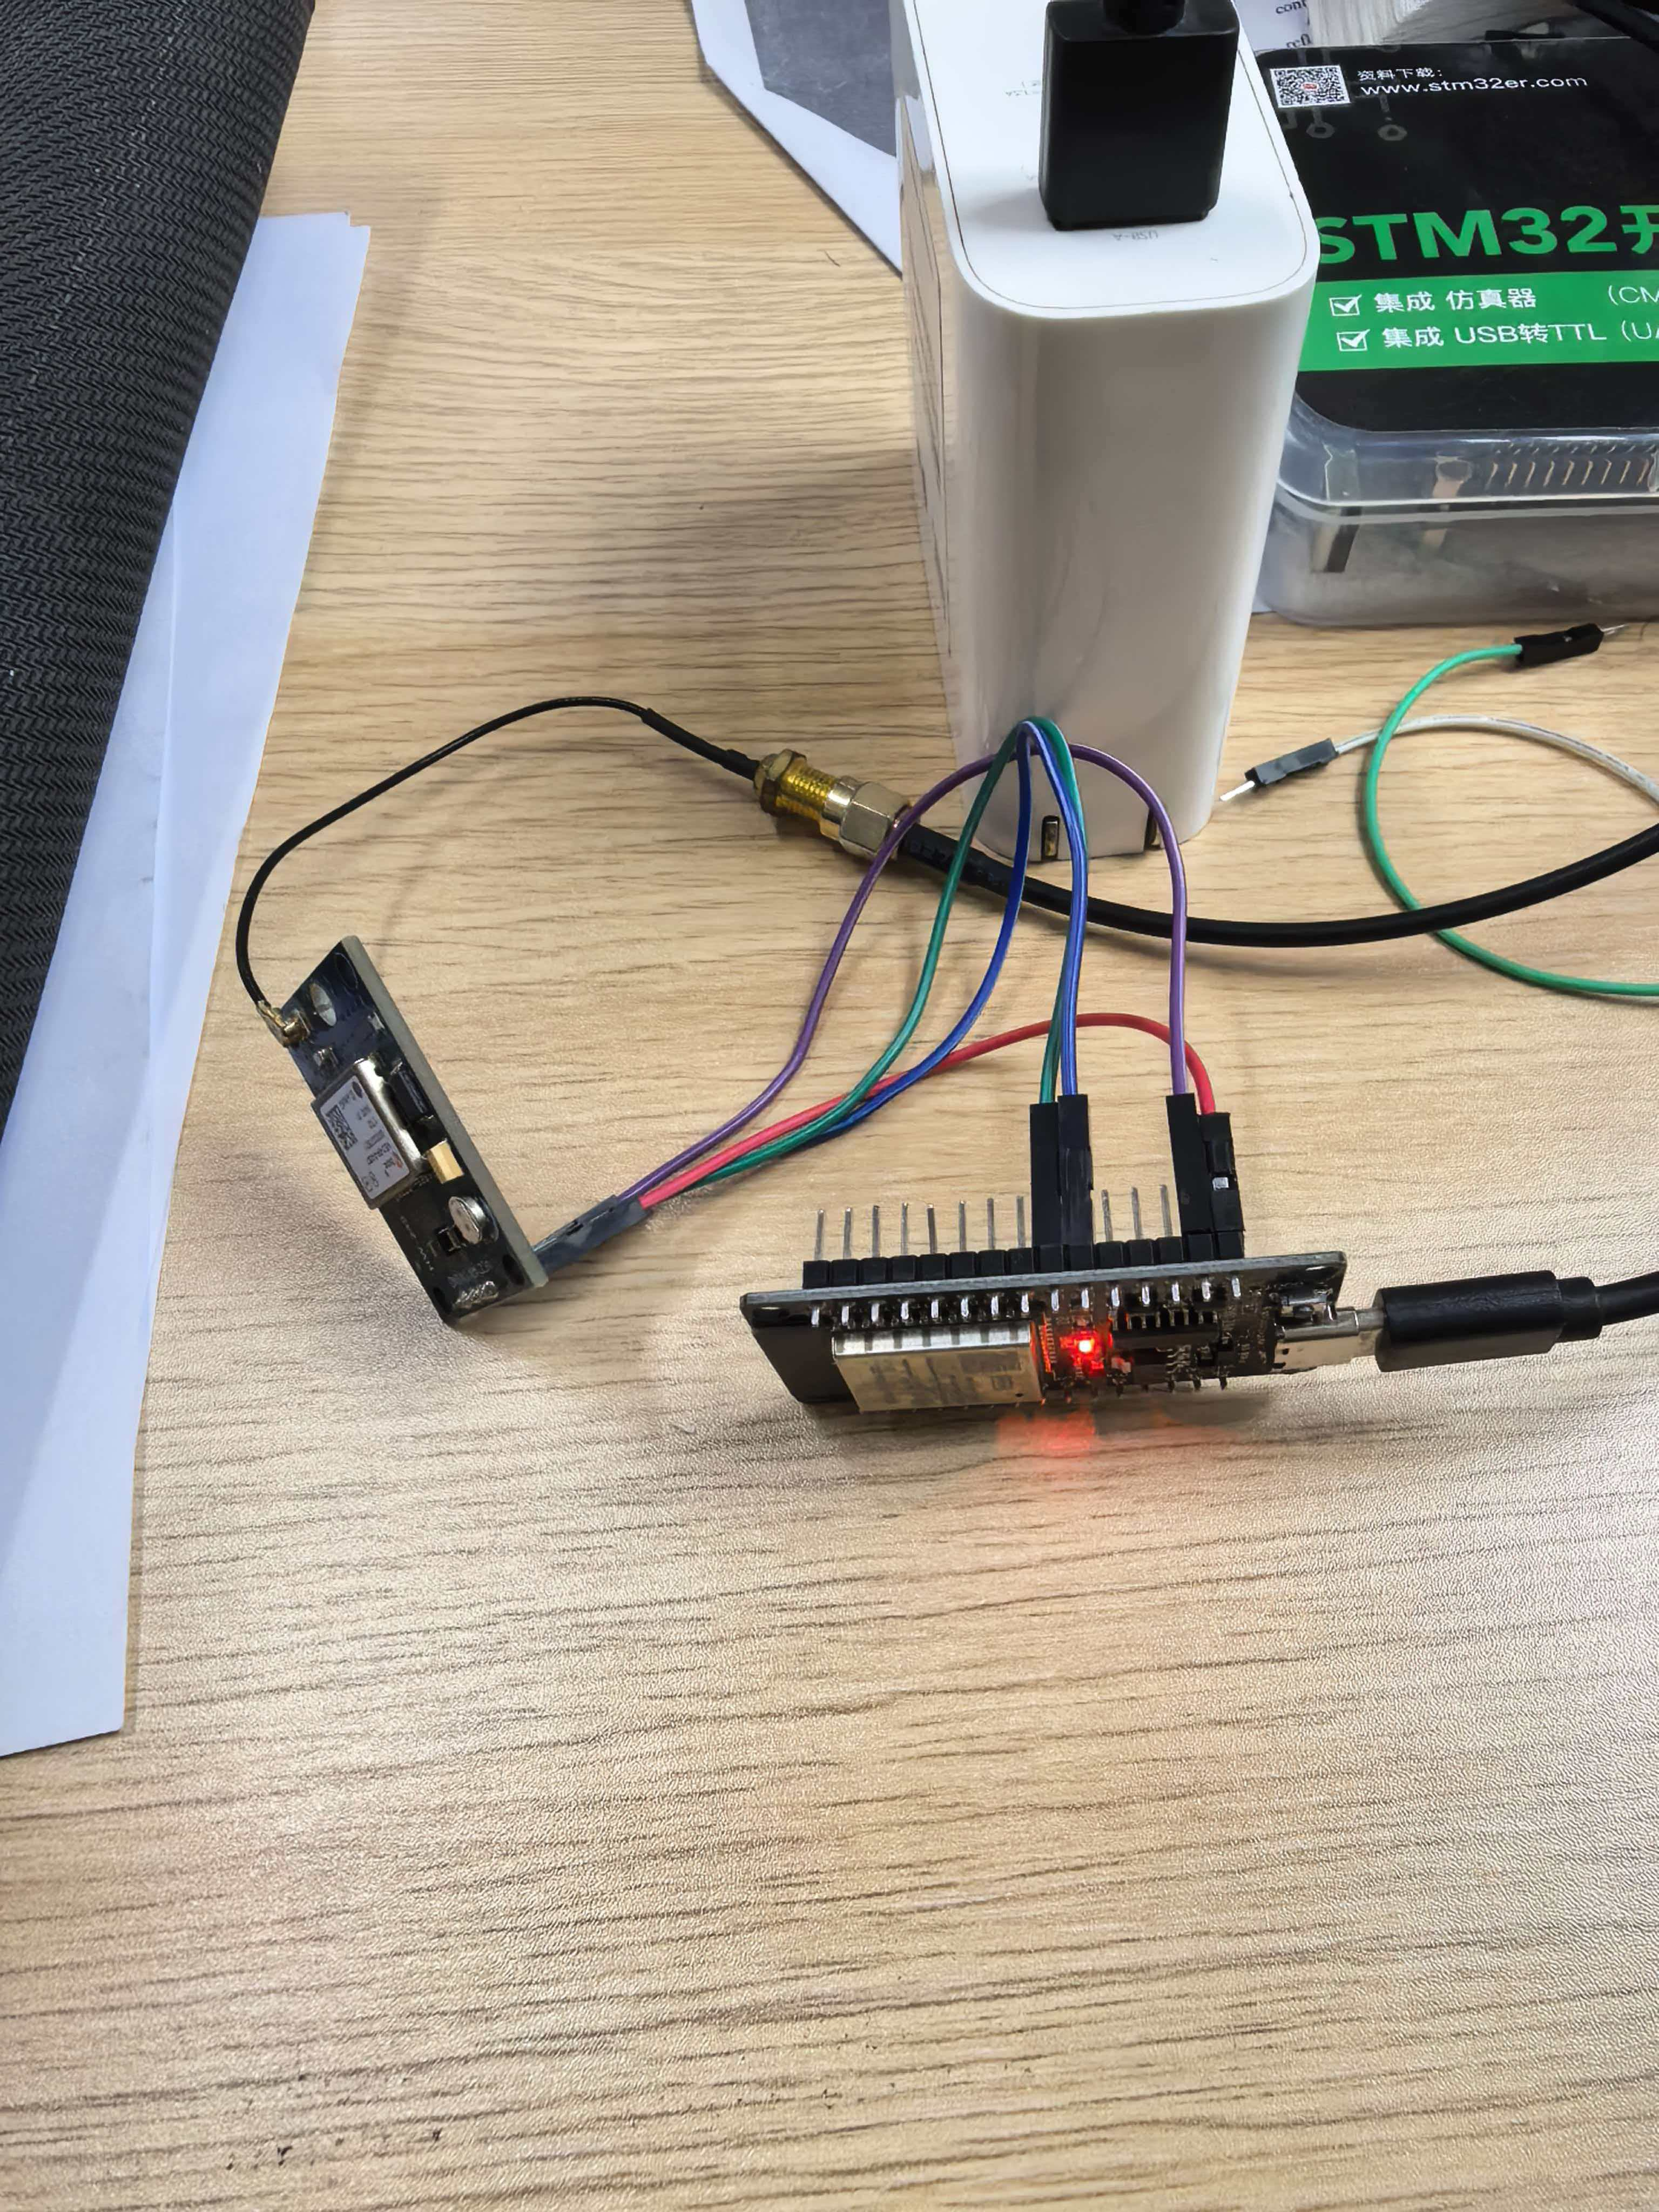
\includegraphics[width=0.64\textwidth,height=0.46\textheight,keepaspectratio]{assets/real_wiring_photo.jpg}
\caption{ESP32 与 GNSS 模块真实接线图}
\label{fig:real-wiring}
\end{figure}

\clearpage
\section{NMEA 协议解析}
\subsection{NMEA 语句结构}
NMEA 0183 语句通常以 \verb|$| 开头，以 \verb|*XX| 校验和结尾。以 GGA 语句为例：

\begin{lstlisting}
$GPGGA,123519,4807.038,N,01131.000,E,1,08,0.9,545.4,M,46.9,M,,*47
\end{lstlisting}

其中 GGA 语句包含 UTC 时间、纬度、经度、定位质量、卫星数、HDOP 和海拔等字段。RMC 语句提供推荐最小定位数据，包含有效状态、经纬度、速度、航向和日期。GSA 语句描述定位模式和 DOP 信息，GSV 语句描述可见卫星信息。本实验解析器支持 GGA、RMC、GSA、GSV 四类语句，其中户外数据分析主要使用 GGA 和 RMC。

\subsection{校验和验证}
本实验没有调用第三方 NMEA 库，而是在 \verb|code/gnss_nmea.py| 中自行实现校验和验证。校验方法是对 \verb|$| 与 \verb|*| 之间的所有字符逐字节 XOR，再与 \verb|*| 后两位十六进制值比较。

\begin{lstlisting}[language=Python]
def nmea_checksum_ok(sentence):
    sentence = sentence.strip()
    if not sentence.startswith("$") or "*" not in sentence:
        return False
    body, checksum_text = sentence[1:].split("*", 1)
    checksum = 0
    for char in body:
        checksum ^= ord(char)
    try:
        expected = int(checksum_text[:2], 16)
    except ValueError:
        return False
    return checksum == expected
\end{lstlisting}

\subsection{经纬度转换}
NMEA 经纬度采用 \verb|ddmm.mmmm| 或 \verb|dddmm.mmmm| 格式，不能直接作为十进制度使用。转换公式为：

\begin{equation}
\text{decimal degree} = \text{degree} + \frac{\text{minute}}{60}
\end{equation}

如果方向标记为 S 或 W，则结果取负值。实现如下：

\begin{lstlisting}[language=Python]
def nmea_latlon_to_deg(value, hemi):
    if not value:
        return None
    raw = float(value)
    degrees = int(raw // 100)
    minutes = raw - degrees * 100
    decimal = degrees + minutes / 60.0
    if hemi in ("S", "W"):
        decimal = -decimal
    return decimal
\end{lstlisting}

\subsection{单元测试}
电脑端运行 \verb|python code\02_test_gnss_parser.py|，测试结果如下：

\begin{lstlisting}
PASS test_checksum_valid
PASS test_checksum_invalid
PASS test_parse_gga_valid
PASS test_parse_gga_no_fix
PASS test_parse_rmc_valid
PASS test_merge_gga_rmc
summary,6/6 passed
\end{lstlisting}

测试覆盖有效校验和、错误校验和、GGA 有效定位、GGA 无定位、RMC 解析和 GGA/RMC 合并，说明步骤二的 NMEA 解析器实现满足任务书要求。

\clearpage
\section{WiFi 数据流设计与实测}
\subsection{系统数据流}
本实验数据流如下：

\begin{center}
\begin{tabular}{c}
GNSS 卫星信号 \\
$\downarrow$ \\
NEO-6M GNSS 模块输出 NMEA \\
$\downarrow$ UART 9600 bps \\
ESP32 校验、解析、合并 GGA/RMC \\
$\downarrow$ WiFi UDP 或 Flash 离线记录 \\
电脑 Python 接收与后处理 \\
$\downarrow$ \\
CSV、folium 地图、matplotlib 图表、Web 可视化 \\
\end{tabular}
\end{center}

\subsection{WiFi UDP 上传设计}
按照任务书 Step 3 要求，本实验实现了 WiFi UDP 上传链路。ESP32 端脚本为 \verb|code/03_wifi_udp_track.py|，电脑端接收脚本为 \verb|code/receiver.py|。ESP32 连接 WiFi 后将解析后的 GNSS 数据封装为 JSON，通过 UDP 发往电脑 8080 端口。电脑端 Python 程序监听 UDP 数据包，打印坐标并保存为 CSV。

选择 UDP 而不是 TCP 的原因是 GNSS 数据约 1 Hz 输出，单条数据短，系统更关注实时性和实现简单性。偶尔丢失一个点不会明显影响整条轨迹分析。

\subsection{WiFi 实测结果}
本实验完成了 WiFi UDP 短时实测，接收文件为：

\begin{lstlisting}
data/track_20260605_212206.csv
\end{lstlisting}

该文件由电脑端 \verb|receiver.py| 监听 UDP 8080 生成。测试共收到 214 条 UDP 数据，其中 88 条包含有效经纬度，能够证明 ESP32 已将解析后的 GNSS 数据通过 WiFi 上传到电脑端并保存为 CSV。测试环境为室内环境，因此后半段出现较多 \verb|quality=0| 的无效定位点，这是 GNSS 信号质量问题，不影响 WiFi 上传链路本身的验证。

\begin{lstlisting}
index,elapsed_ms,time,date,status,quality,lat,lon,alt,sats,hdop,speed_knots,course_deg
0,37787,132504.00,,V,1,26.03073,119.1932,40.9,4,5.81,,
1,38789,132505.00,,V,1,26.03072,119.1932,39.5,4,5.81,,
2,39786,132506.00,050626,A,1,26.03072,119.1932,37.1,4,5.82,2.462,
\end{lstlisting}

\section{户外采集实验}
\subsection{采集方案}
实际户外采集时，为避免移动过程中 WiFi 覆盖不稳定、电脑携带不方便、UDP 丢包等问题，本实验采用 ESP32 Flash 离线记录作为主采集方案。采集脚本为 \verb|code/05_flash_track_logger.py|，ESP32 上电后等待有效定位，然后自动记录 CSV 到内部 Flash。采集结束后通过 mpremote 取回电脑，主实验数据保存为：

\begin{lstlisting}
data/track_flash_outdoor_001.csv
\end{lstlisting}

户外采集时按照任务书安全要求执行：采集过程中持续关注设备状态和路况；ESP32、NEO-6M 和充电宝放入背包；天线朝上；手机运动 App 同步记录 GPX；关键拐点手动记录时间。

\subsection{采集结果统计}
本次户外采集时间约为 UTC 12:05:02 到 12:22:34。ESP32 有效定位段约为 UTC 12:05:02 到 12:21:55。统计结果如表 \ref{tab:outdoor-summary} 所示。

\begin{table}[H]
\centering
\caption{户外 GNSS 数据统计}
\label{tab:outdoor-summary}
\begin{tabular}{lr}
\toprule
指标 & 数值 \\
\midrule
总采样点数 & 1051 \\
有效定位点数 & 863 \\
有效定位率 & 82.11\% \\
平均 HDOP & 2.65 \\
平均卫星数 & 4.00 \\
最少卫星数 & 4 \\
最多卫星数 & 4 \\
\bottomrule
\end{tabular}
\end{table}

有效定位率为 82.11\%，超过任务书要求的 70\%。总采样点数 1051，也超过 500 点要求。后半段出现部分无效定位点，说明路线末端可能进入了遮挡较强的位置，例如楼下、室内入口、树木密集区或背包遮挡严重的位置。

\clearpage
\section{可视化结果}
\subsection{实测轨迹地图}
本实验使用 \verb|code/plot_track.py| 生成 folium 轨迹地图 \verb|data/track.html|。为了便于 LaTeX 报告展示，另根据实测 CSV 生成静态轨迹图，如图 \ref{fig:esp-track} 所示。图中红线为 ESP32 有效定位轨迹，点颜色根据 HDOP 变化，起点和有效定位终点分别标记。

\begin{figure}[H]
\centering
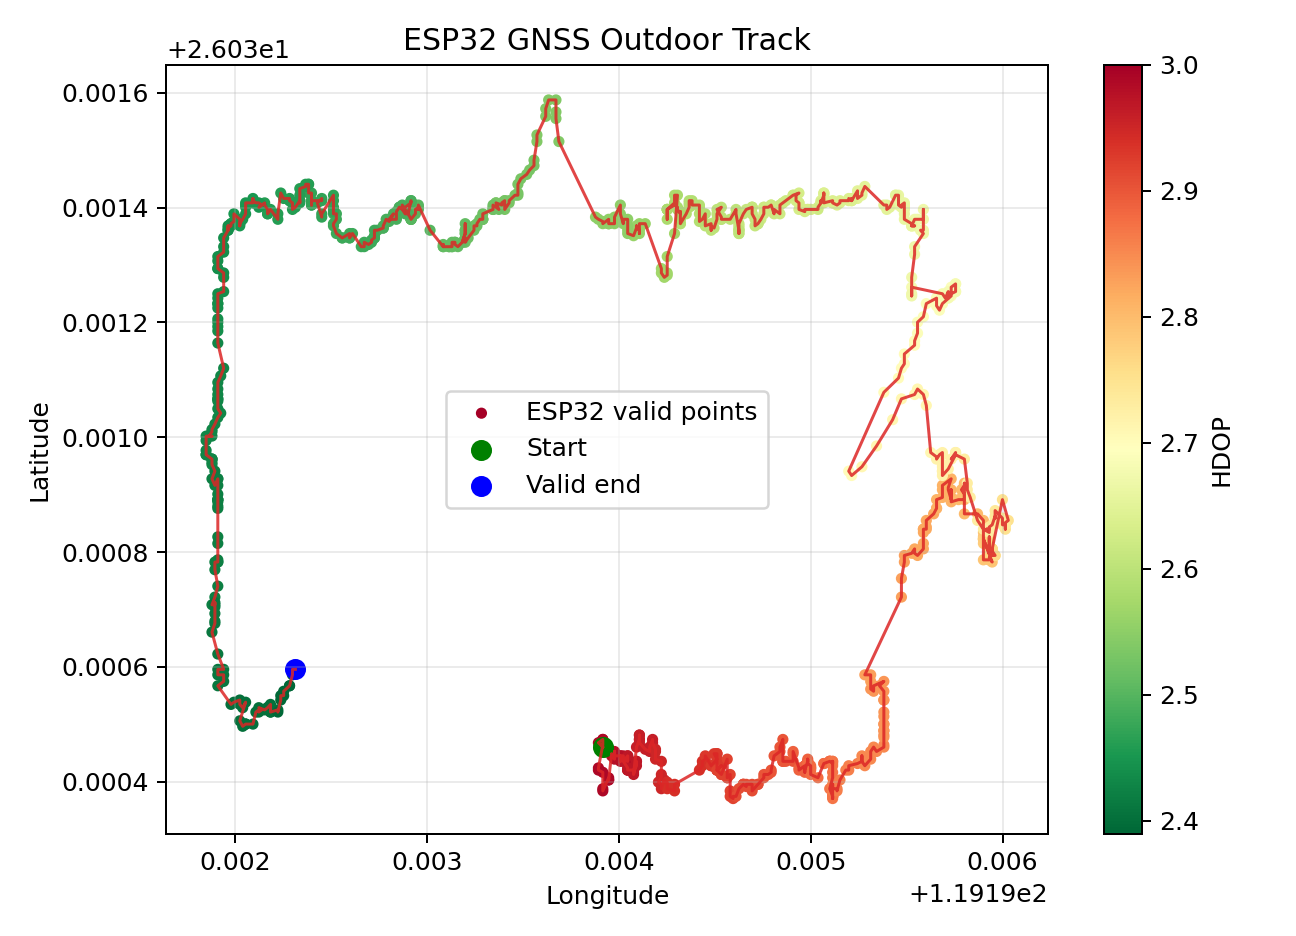
\includegraphics[width=0.82\textwidth,height=0.48\textheight,keepaspectratio]{assets/esp32_outdoor_track_map.png}
\caption{ESP32 GNSS 户外实测轨迹地图截图}
\label{fig:esp-track}
\end{figure}

\subsection{定位质量统计图}
图 \ref{fig:hdop-sats} 展示 HDOP 与卫星数随时间变化。HDOP 值越小，水平定位几何条件通常越好。本次实验平均 HDOP 为 2.65，属于可用但不算优秀。卫星数长期为 4 颗，说明采集环境下可见卫星数较少，定位稳定性容易受遮挡影响。

\begin{figure}[H]
\centering
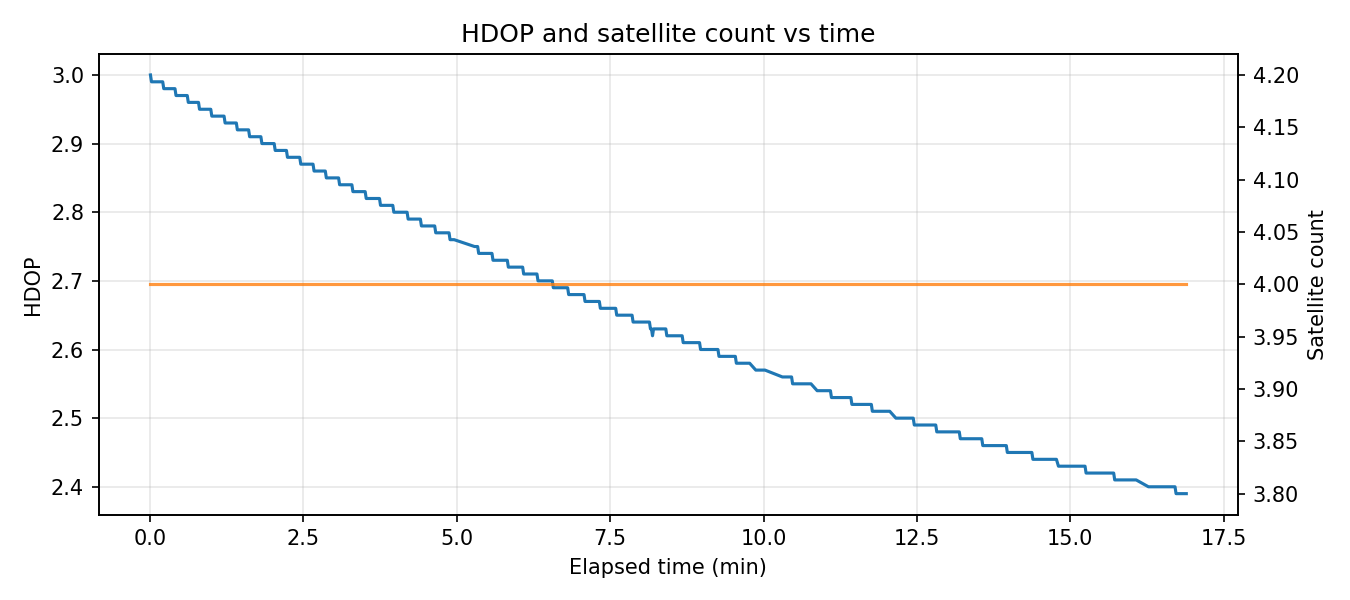
\includegraphics[width=0.84\textwidth,height=0.36\textheight,keepaspectratio]{assets/hdop_satellite_time_series.png}
\caption{HDOP 与卫星数随时间变化}
\label{fig:hdop-sats}
\end{figure}

\begin{figure}[H]
\centering
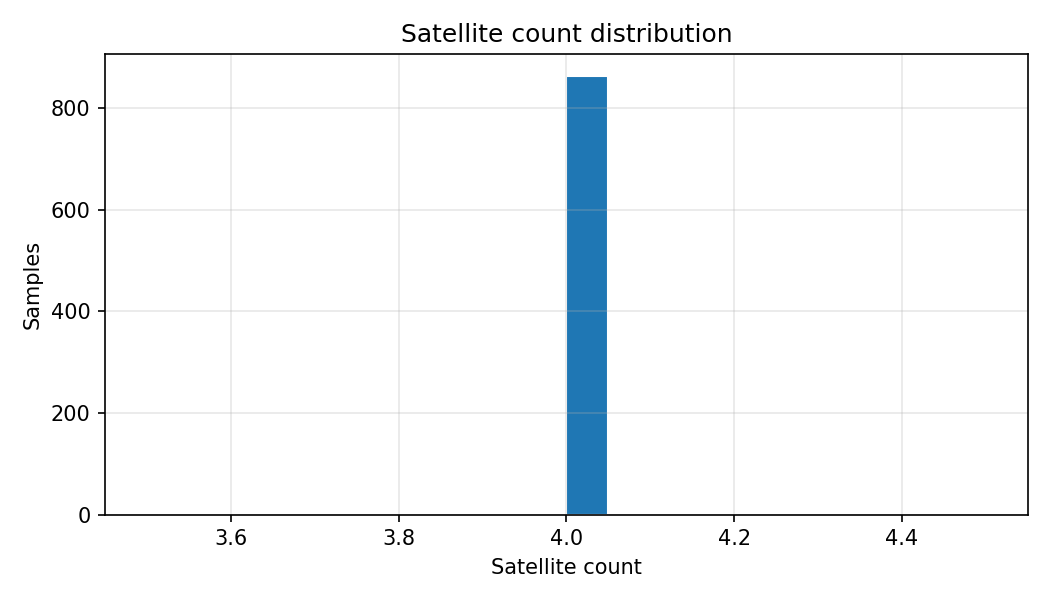
\includegraphics[width=0.64\textwidth,height=0.32\textheight,keepaspectratio]{assets/satellite_count_distribution.png}
\caption{卫星数分布}
\label{fig:sat-dist}
\end{figure}

\clearpage
\section{手机 GPS 对比分析}
\subsection{手机参考轨迹}
采集过程中手机运动 App 同步记录户外运动路线，App 显示路线约 0.94 km，时间为 2026 年 6 月 5 日 20:04 左右，如图 \ref{fig:phone-app-track} 所示。该截图作为手机参考轨迹的实测证据。原始手机轨迹文件包含个人位置隐私，不作为最终提交文件；报告中保留已经生成的叠加地图、统计摘要和对比图。

\begin{figure}[H]
\centering
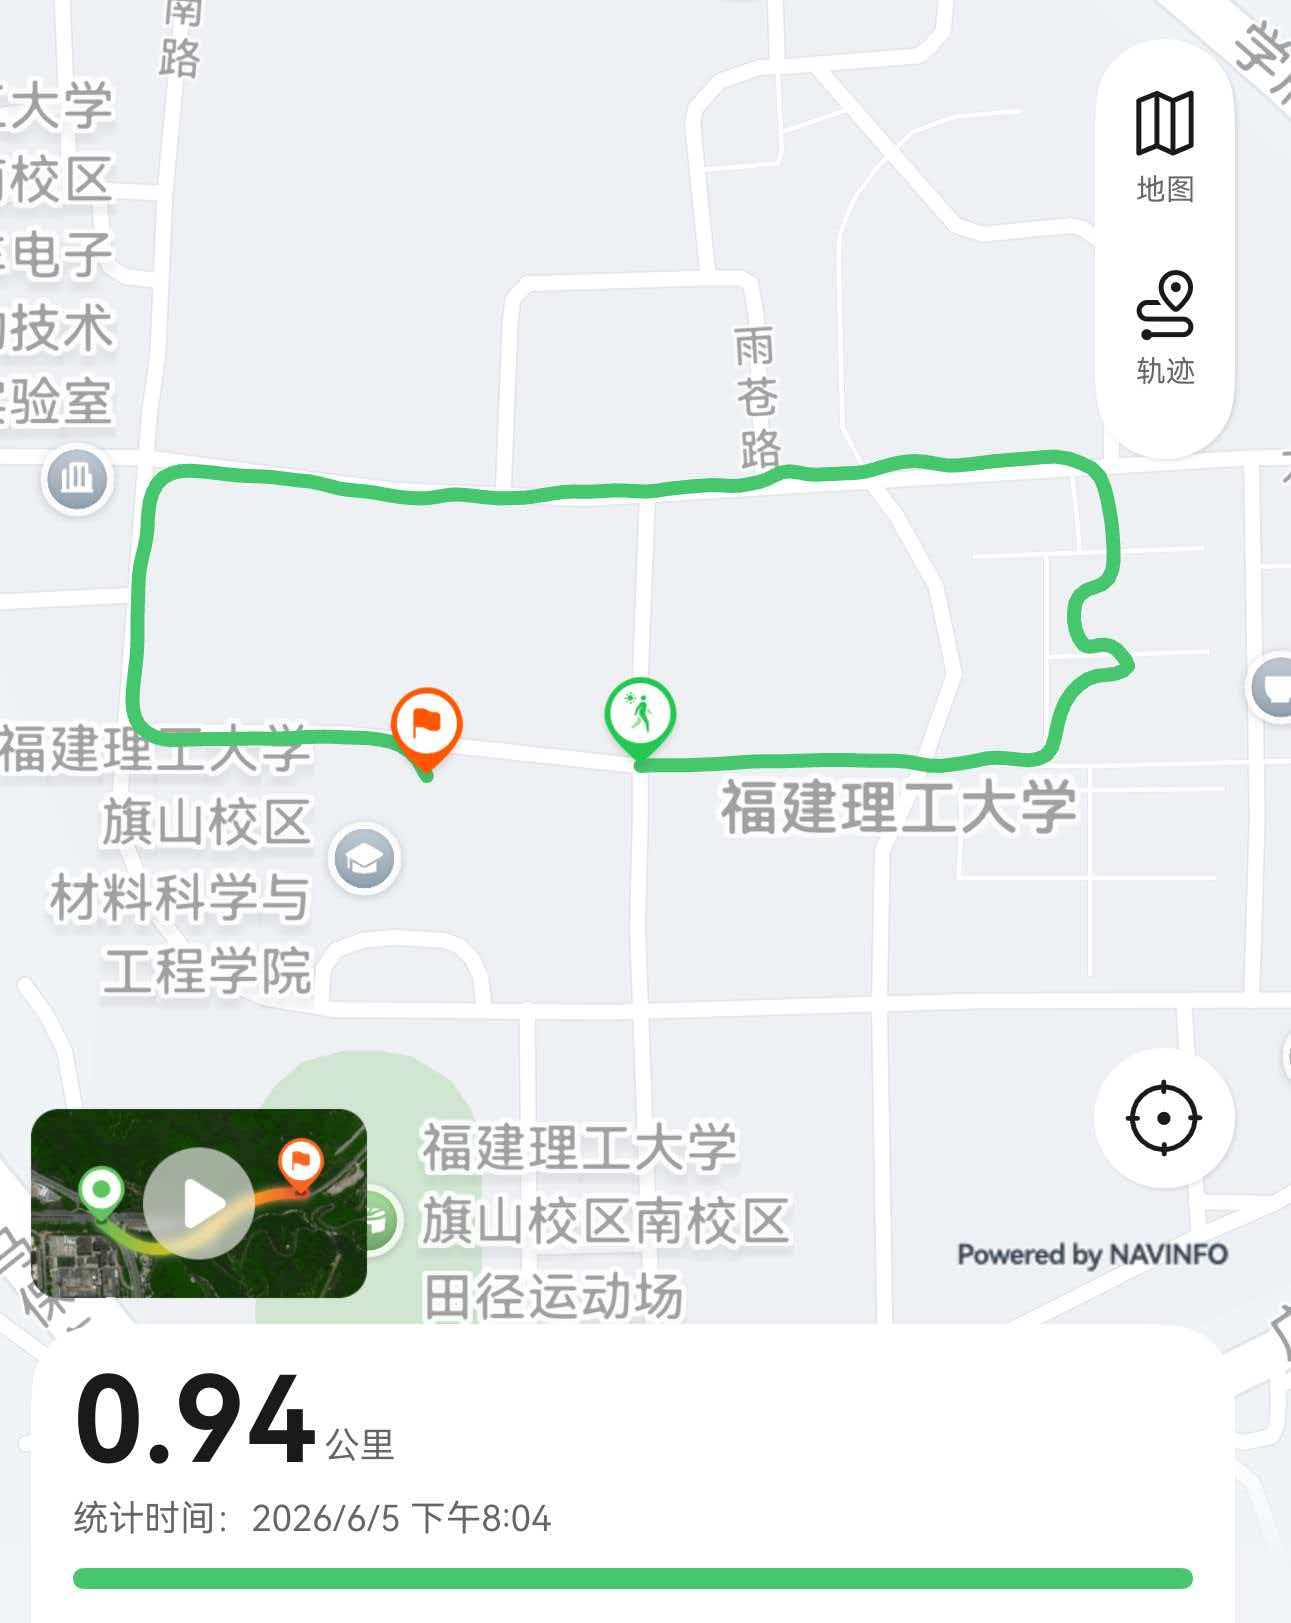
\includegraphics[width=0.48\textwidth,height=0.42\textheight,keepaspectratio]{assets/phone_app_track_screenshot.jpg}
\caption{手机运动 App 同步记录的户外轨迹截图}
\label{fig:phone-app-track}
\end{figure}

本实验使用 \verb|code/compare_esp_phone.py| 将手机参考轨迹与 ESP32 轨迹叠加，生成 folium 文件 \verb|data/esp_phone_overlay.html|，并生成静态对比图，如图 \ref{fig:phone-overlay} 所示。

\begin{figure}[H]
\centering
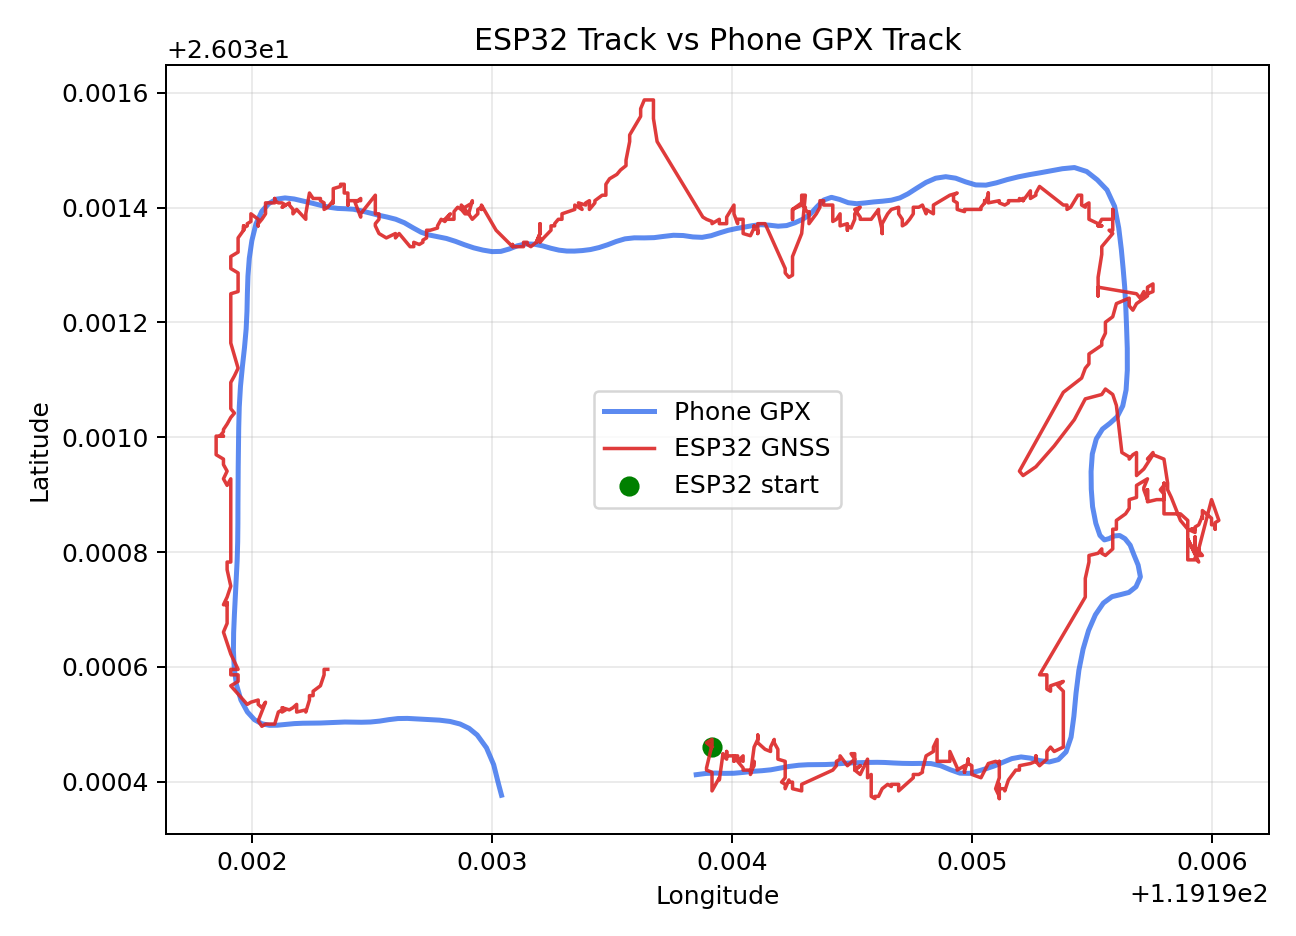
\includegraphics[width=0.82\textwidth,height=0.46\textheight,keepaspectratio]{assets/esp32_phone_overlay_map.png}
\caption{ESP32 轨迹与手机 GPX 轨迹叠加对比}
\label{fig:phone-overlay}
\end{figure}

\subsection{对比结果}
手机参考轨迹在本地处理时发现部分时间戳异常：真实路线几何点带有 1970 年异常时间，而后续 2026 年时间点对应固定坐标。因此本实验不采用严格时间同步误差计算，而采用空间最近距离方式评估两条轨迹差异。统计结果如表 \ref{tab:phone-compare} 所示。

\begin{table}[H]
\centering
\caption{ESP32 与手机轨迹空间对比}
\label{tab:phone-compare}
\begin{tabular}{lr}
\toprule
指标 & 数值 \\
\midrule
ESP32 原始样本 & 1051 \\
ESP32 有效样本 & 863 \\
手机 GPX 点数 & 573 \\
ESP32 轨迹长度 & 1536.99 m \\
手机轨迹长度 & 873.23 m \\
最近距离均值 & 6.37 m \\
最近距离中位数 & 4.07 m \\
最近距离 95\% 分位数 & 23.57 m \\
最大最近距离 & 34.47 m \\
\bottomrule
\end{tabular}
\end{table}

\begin{figure}[H]
\centering
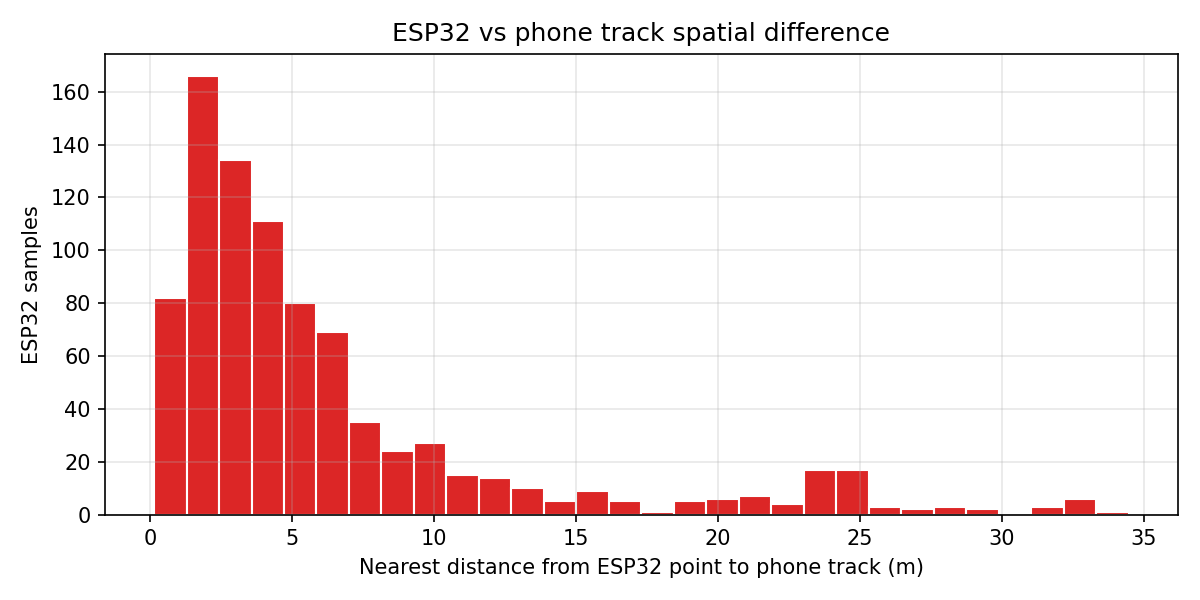
\includegraphics[width=0.74\textwidth,height=0.34\textheight,keepaspectratio]{assets/esp_phone_nearest_distance.png}
\caption{ESP32 有效点到手机轨迹的最近距离分布}
\end{figure}

从结果看，ESP32 轨迹与手机轨迹大多数路段比较接近。最近距离中位数为 4.07 m，符合普通单点 GNSS 米级定位的典型表现。少数点偏差较大，可能来自楼宇遮挡、多路径反射、手机轨迹平滑、GPX 时间戳异常或 ESP32 天线姿态变化。

\clearpage
\section{质量分析}
\subsection{有效定位率}
本次 ESP32 总采样点数为 1051，有效定位点为 863，有效率为 82.11\%。该结果满足实验要求。无效点主要出现在后半段，说明采集路线中存在信号质量下降区域。与手机轨迹对比可见，ESP32 在多数路段可以反映真实运动趋势，但在遮挡较强区域会出现漂移或失锁。

\subsection{HDOP 分析}
一般情况下，HDOP 小于 1 认为优秀，1 到 2 较好，2 到 5 可用但误差可能增大，大于 5 则较差。本次户外平均 HDOP 为 2.65，处于可用范围但并不优秀。由于有效定位样本中卫星数主要为 4 颗，说明卫星几何分布较弱，定位容易受到遮挡和多路径影响。

\subsection{卫星数分析}
4 颗卫星是三维定位所需的最低可用数量。三维坐标加接收机钟差共有 4 个未知数，需要至少 4 颗卫星提供伪距约束。因此，一旦遮挡导致可见卫星数少于 4 颗，定位就会变为无效。实验中出现的 \verb|quality=0| 点与这一原理相符。

\subsection{室内与室外对比}
本实验补充了室外路线与室内环境定位质量对比，使用室外主实验文件 \verb|data/track_flash_outdoor_001.csv| 与室内 WiFi 短测文件 \verb|data/track_20260605_212206.csv|。结果如表 \ref{tab:env-compare} 和图 \ref{fig:env-compare} 所示。

\begin{table}[H]
\centering
\caption{室内与室外定位质量对比}
\label{tab:env-compare}
\begin{tabular}{lrr}
\toprule
指标 & 室外路线 & 室内短测 \\
\midrule
总样本数 & 1051 & 214 \\
有效定位点数 & 863 & 88 \\
有效定位率 & 82.11\% & 41.12\% \\
平均 HDOP（有效点） & 2.65 & 5.91 \\
平均卫星数（有效点） & 4.00 & 4.09 \\
无效点数 & 188 & 126 \\
\bottomrule
\end{tabular}
\end{table}

\begin{figure}[H]
\centering
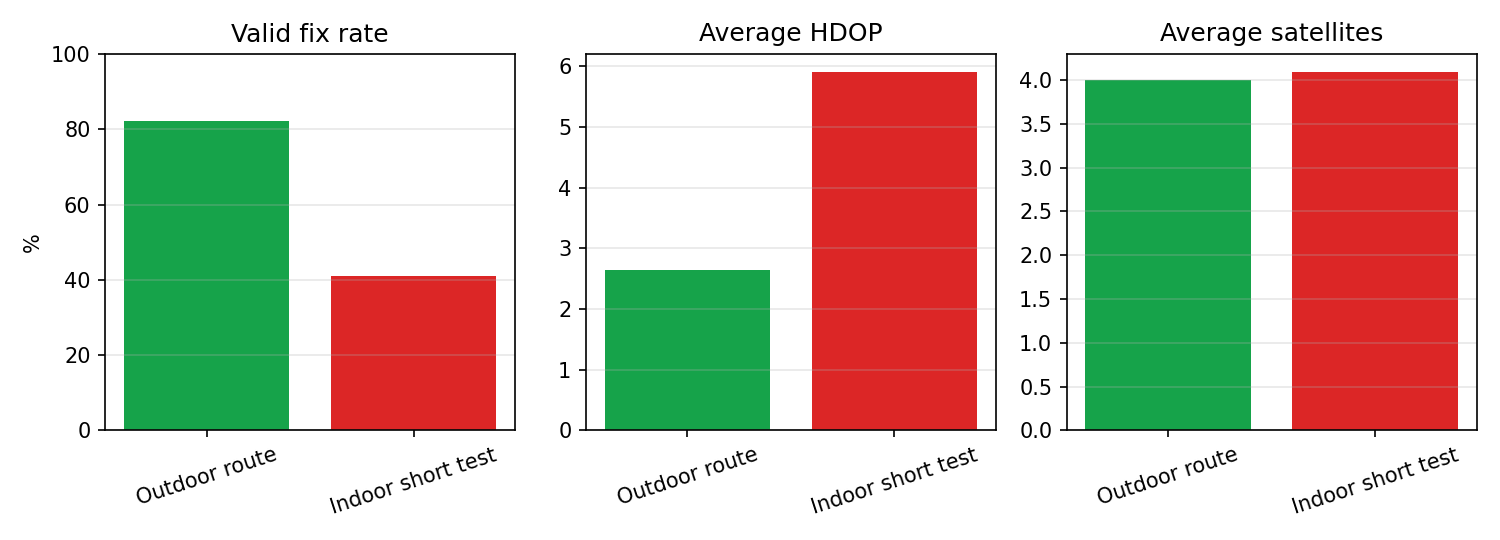
\includegraphics[width=0.76\textwidth,height=0.36\textheight,keepaspectratio]{assets/indoor_outdoor_quality_compare.png}
\caption{室外与室内定位质量对比图}
\label{fig:env-compare}
\end{figure}

从对比结果看，室内短测有效率下降到 41.12\%，平均 HDOP 上升到 5.91，说明室内墙体和楼板明显削弱 GNSS 信号。即使有效点平均卫星数接近 4 颗，由于卫星数刚好处在最低定位门槛附近，定位质量仍然很脆弱。这一结果直观说明了 GNSS 在室内环境中的局限性。

\clearpage
\section{挑战项：实时 Web 可视化}
本实验实现了实时 Web 可视化功能，代码文件为 \verb|code/realtime_web_visualizer.py|。该程序使用 Flask 提供网页页面，使用 WebSocket 推送 GNSS 数据，并使用 Leaflet 在浏览器中动态绘制轨迹。程序支持 UDP 实时模式和 CSV 回放模式。

\begin{lstlisting}
python code\realtime_web_visualizer.py --mode udp
python code\realtime_web_visualizer.py --mode replay --csv data\track_flash_outdoor_001.csv
\end{lstlisting}

本次报告采用 CSV 回放模式作为验证证据。程序读取户外实测文件 \verb|data/track_flash_outdoor_001.csv|，再按采样顺序通过 WebSocket 逐点推送到浏览器端。启动后打开 \verb|http://127.0.0.1:5000|，网页中显示连接状态、实时样本数、当前坐标、定位质量、卫星数和 HDOP，并用 Leaflet 地图动态绘制轨迹线。轨迹点按 HDOP 着色：绿色表示较好，橙色表示一般，红色表示较差。

\begin{figure}[H]
\centering
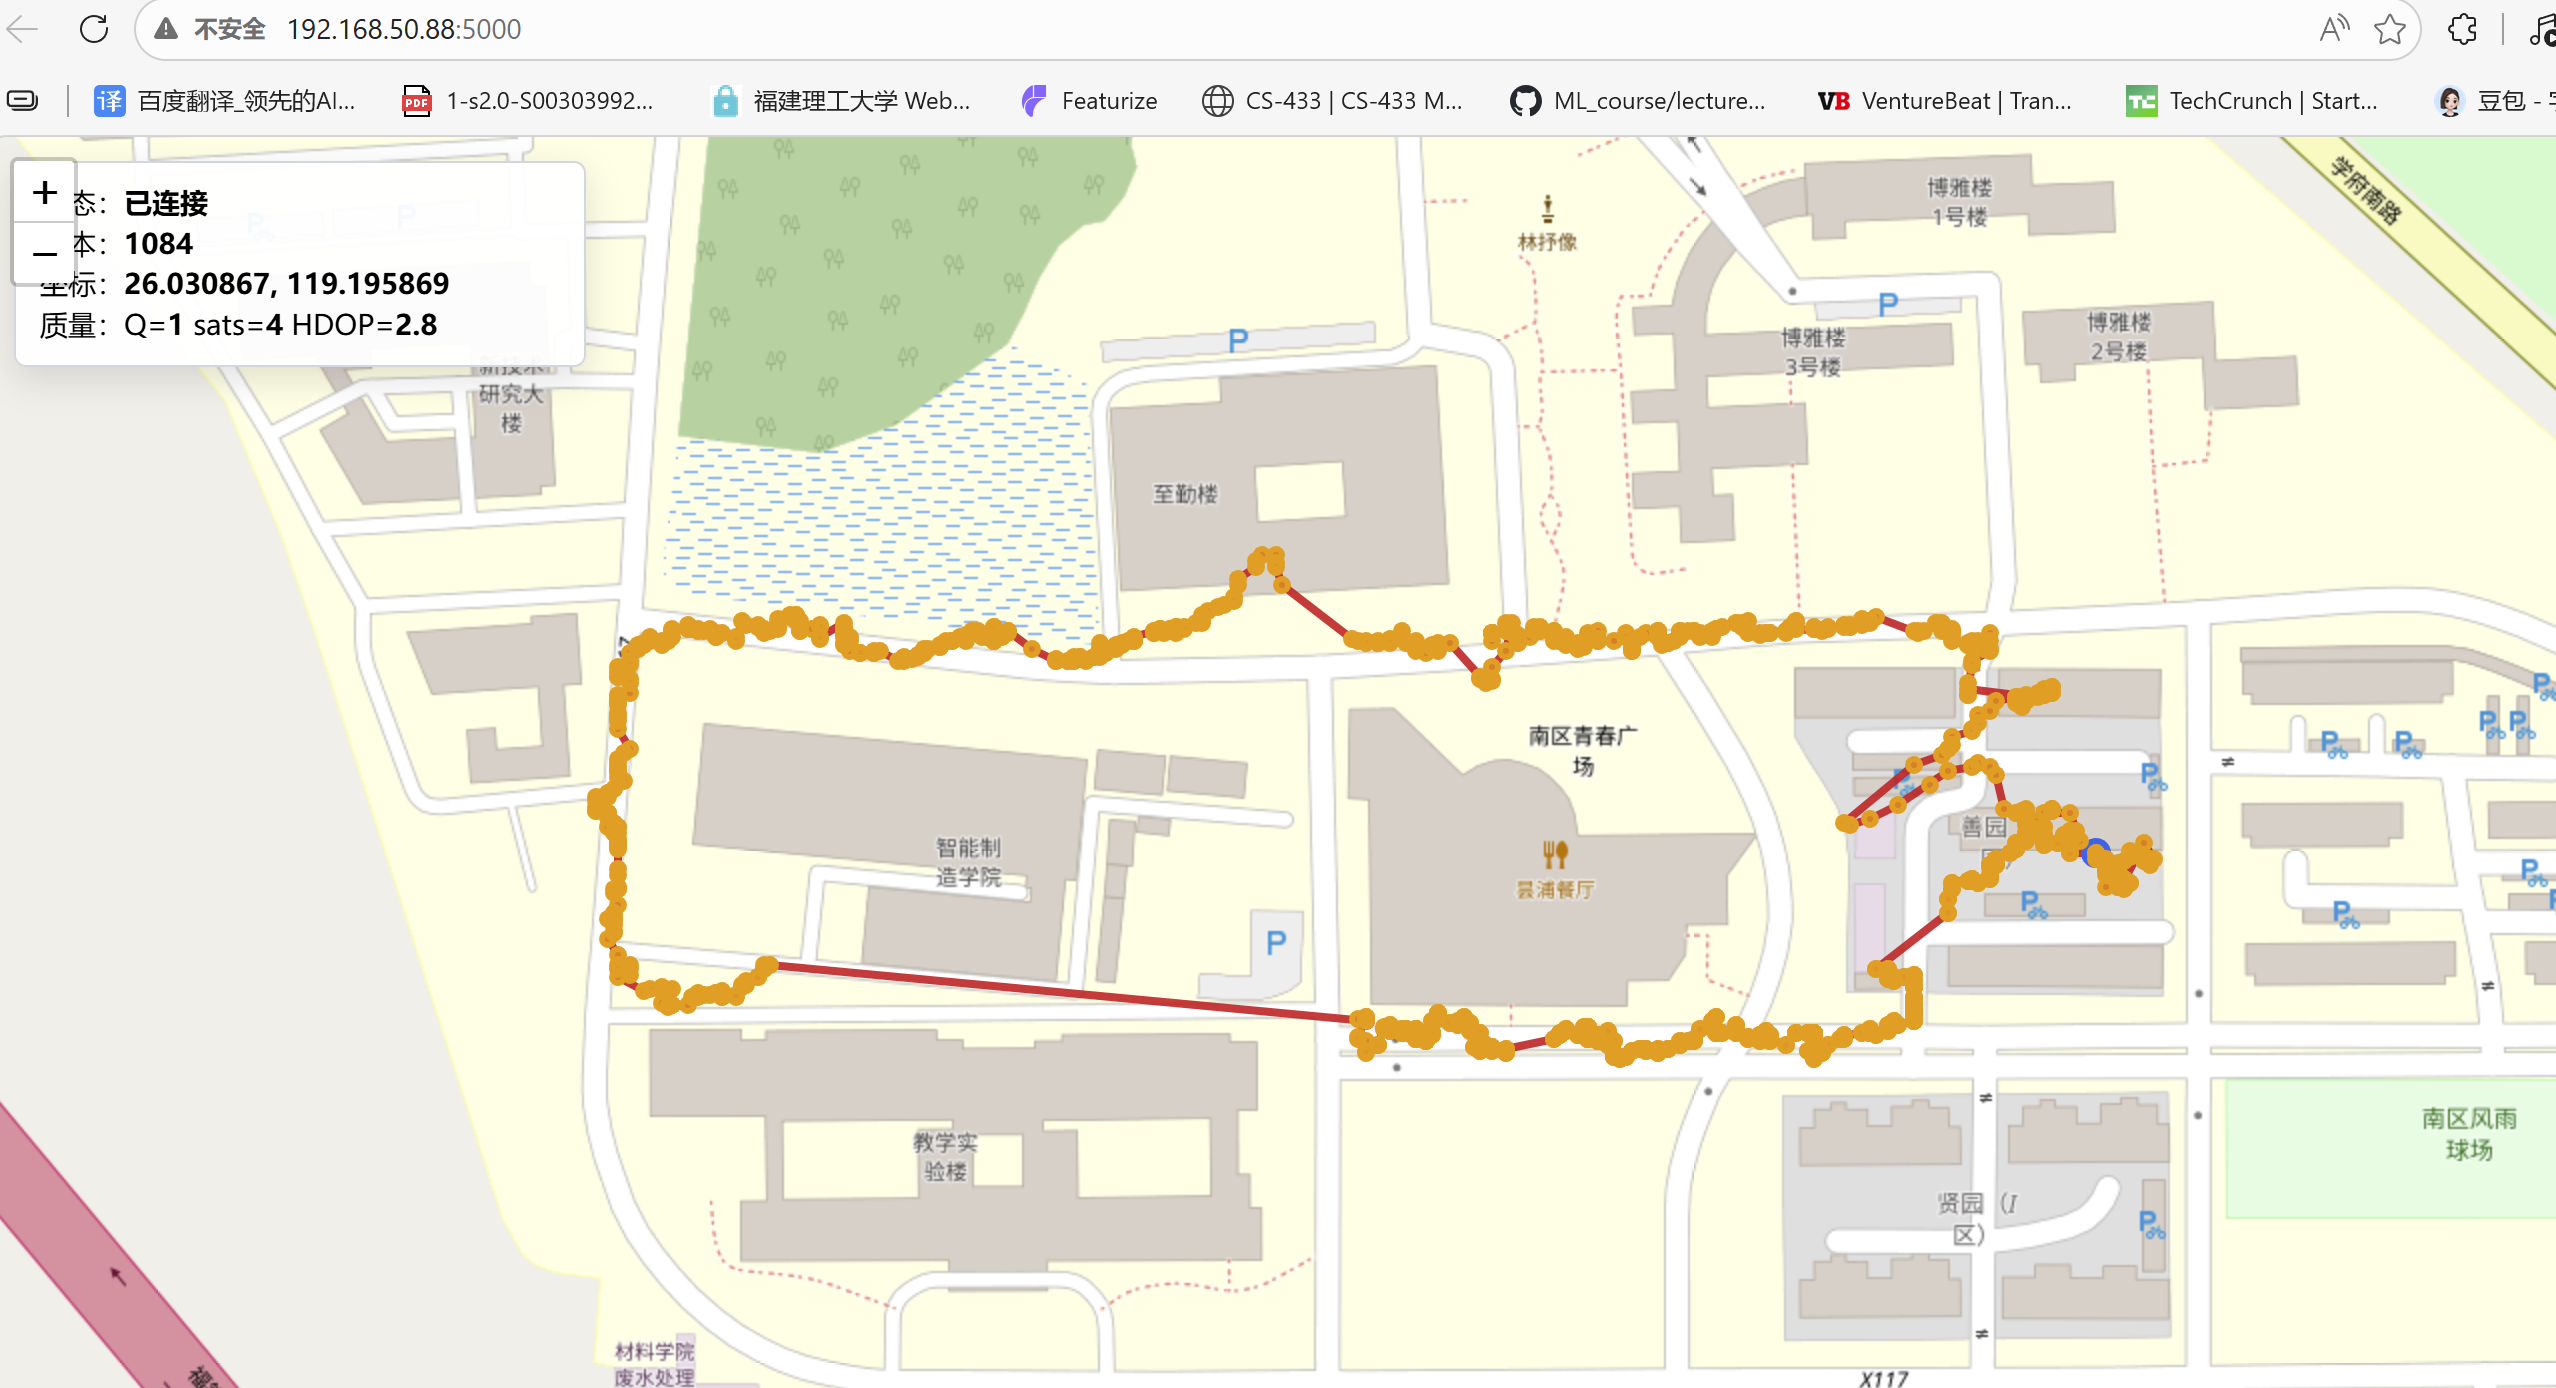
\includegraphics[width=0.84\textwidth,height=0.46\textheight,keepaspectratio]{assets/realtime_web_replay.png}
\caption{户外实测轨迹的 WebSocket 实时回放可视化页面}
\label{fig:web-replay}
\end{figure}

图 \ref{fig:web-replay} 中页面状态为“已连接”，样本数已经动态更新到 1084，说明网页端正在持续接收后端推送的数据并绘制轨迹。虽然该截图使用的是已采集 CSV 的回放模式，但数据流仍然经过 Flask 页面、WebSocket 推送和 Leaflet 动态绘制，展示逻辑与 UDP 实时接收模式一致。因此，该截图可以作为任务书挑战项“实时 Web 可视化（Flask + WebSocket + Leaflet）”的实测证据。

\section{RTKLIB 对比说明}
任务书中 RTKLIB 为挑战任务和加分项，需要使用 u-center 记录 UBX 原始观测数据，再通过 RTKLIB convbin 转 RINEX，并使用 rnx2rtkp 进行后处理。本次实验没有获得 UBX/RINEX 原始观测文件，也没有完成 RTKLIB `.pos` 解算，因此不伪造 RTKLIB 结果。报告保留该说明，后续若具备 USB-TTL、u-center 和 RTKLIB 工具链，可继续补充该项。

\clearpage
\section{思考题作答}
\subsection{GPS 单点定位为什么通常只有米级精度？}
单点 GPS 定位精度受多个物理误差源限制。首先，民用 GPS L1 C/A 码的码片速率有限，接收机通过相关峰估计伪距时会产生码跟踪误差。其次，卫星钟差、星历误差、电离层延迟、对流层延迟都会改变信号传播时间，使接收机把时间误差误认为距离误差。第三，接收机天线附近的墙面、玻璃、金属结构会产生多路径反射，反射信号路径更长，会使伪距偏大。最后，卫星几何分布会通过 DOP 因子放大伪距误差。如果卫星集中在天空一侧，即使每颗卫星伪距误差不大，最终水平位置误差也可能明显增大。因此普通单频单点定位通常只能达到数米精度。

\subsection{HDOP 的几何意义是什么？}
HDOP 是水平精度因子，反映卫星几何分布对水平定位误差的放大作用。可以把定位理解成多个距离约束的交会问题。如果卫星分布在天空不同方向，伪距约束的交会角度较好，误差椭圆较小，水平定位更稳定，HDOP 较低。如果卫星集中在同一侧，约束方向相似，交会角度差，微小伪距误差就会把最终位置推得很远，HDOP 增大。因此 HDOP 不直接表示米级误差，而是表示几何结构对测距误差的放大倍数。开阔地通常 HDOP 较低，高楼旁、树下、城市峡谷中 HDOP 容易变高。

\subsection{楼下定位变差主要是什么误差？如何缓解？}
楼下定位变差主要来自遮挡和多路径效应。建筑物会遮挡部分天空，使接收机可见卫星数量减少，卫星几何分布变差。同时，墙面、玻璃幕墙、金属结构会反射 GNSS 信号，接收机可能同时收到直达波和反射波。反射波路径更长，会导致伪距偏大，从而造成位置漂移。缓解方法包括：选择开阔位置采集，让天线远离墙面并朝上；使用更好的有源天线或带地板的天线；使用多系统多频接收机提高可见卫星数量；融合 IMU、地图、轮速计等信息进行约束；在后处理中剔除 HDOP 高、卫星数低或速度异常的数据点。

\subsection{北斗与 GPS 有什么关键区别？为什么中国必须建设自己的 GNSS？}
GPS 是美国建设的全球卫星导航系统，北斗是中国自主建设的全球卫星导航系统。两者都能提供定位、测速和授时服务，但北斗拥有自主星座、自主信号体制、自主地面控制系统，并具备短报文等特色服务。定位导航授时能力是交通、电力、通信、金融、测绘、农业、应急和国防的重要基础设施。如果完全依赖国外系统，在极端情况下可能面临服务降级、区域限制或不可控风险。因此，中国建设北斗不仅是技术发展需求，也是国家安全、产业安全和关键基础设施安全的需求。自主 GNSS 能提升系统韧性，也能推动导航芯片、接收机、测绘和智能交通产业发展。

\subsection{RTK 厘米级定位适合哪些场景？哪些场景属于过度使用？}
RTK 使用基准站和流动站的差分观测，结合载波相位测量，可显著削弱卫星钟差、星历误差和大气延迟等共同误差，实现厘米级定位。它适合工程测量、无人机测绘、精准农业、自动驾驶测试、机器人巡检、港口自动化、形变监测等对绝对位置精度要求很高的场景。但在普通手机导航、跑步轨迹记录、物流粗定位、校园签到、一般 IoT 设备定位中，米级精度通常已经足够。此时使用 RTK 会增加硬件成本、网络服务依赖、初始化复杂度和维护成本，属于过度使用。工程中应根据场景精度需求、成本和可靠性综合选择定位方案。

\subsection{GPS 信号可以被伪造，如何防范 GPS 欺骗？}
GPS 信号公开且到达地面时功率很低，因此攻击者可能发射伪造信号诱导接收机输出错误位置。防护可以从信号层、系统层和融合层进行。信号层可监测异常信号强度、相关峰形状、载噪比变化和到达角；多天线接收机还能利用相位差判断信号方向是否合理。系统层可同时使用 GPS、北斗、Galileo、GLONASS 等多系统，检查不同系统解算结果是否一致。融合层可结合 IMU、轮速计、视觉、地图、气压计等传感器，如果 GNSS 位置与惯性预测或环境约束严重冲突，就降低 GNSS 权重或触发告警。对高安全场景，还应使用加密认证信号、干扰检测和异常轨迹识别。

\clearpage
\section{AI 协作记录}
本实验使用 AI 作为编程和报告整理辅助工具，但实验数据、硬件接线、户外路线采集和手机运动 App 轨迹均由本人实际完成。AI 协作主要体现在以下几个方面。

\begin{enumerate}
\item \textbf{任务书拆解与方案选择。} 根据老师发布的《实验三 GNSS驱动与高精度定位》任务书，AI 协助将实验拆分为硬件接线、NMEA 接收、协议解析、WiFi 上传、户外采集、folium 可视化、手机轨迹对比、实时 Web 可视化和室内外定位质量分析等模块。由于实际硬件为 ESP32，最终采用 MicroPython 完成嵌入式端实现，并在报告中如实说明实现环境。
\item \textbf{代码组织与调试辅助。} AI 协助编写和整理了自写 NMEA 解析器、ESP32 端串口采集脚本、WiFi UDP 上传脚本、Flash 本地记录脚本、电脑端 UDP 接收程序和 Python 后处理脚本。解析器没有调用现成 NMEA 库，而是自行完成校验和、字段拆分、GGA/RMC 解析和 ddmm.mmmm 到十进制度的转换。
\item \textbf{验证与结果整理。} AI 协助设计单元测试并整理测试输出，当前解析器测试结果为 6/6 PASS。户外主数据文件包含 1051 个采样点，其中 863 个有效定位点，有效率为 82.11\%。AI 协助生成 folium 地图、HDOP/卫星数统计图、ESP32 与手机 GPX 对比图，以及室内/室外定位质量对比图。
\item \textbf{报告撰写与诚信边界。} AI 协助将实验过程整理为 LaTeX 报告，并补充思考题初稿和图表说明。对于没有真实完成的 RTKLIB 后处理，本报告没有伪造 `.pos` 或厘米级定位结果，而是如实写明缺少 UBX/RINEX 原始观测文件，后续可继续完成该挑战项。
\end{enumerate}

通过 AI 协作，本实验提高了代码组织、数据分析和报告排版效率；同时保留了实验真实性，所有关键结论均来自本人采集的 ESP32 GNSS 数据、WiFi 短测数据和手机 GPX 对比数据。

\section{实验总结}
本实验完成了 ESP32 与 GNSS 模块的连接、NMEA 数据接收、自写解析、WiFi UDP 上传、户外数据采集、地图可视化和质量分析。通过单元测试验证了解析器的正确性；通过 WiFi 短测证明 ESP32 能将解析后的坐标上传到电脑端；通过户外采集获得 1051 条 ESP32 GNSS 数据，其中 863 条为有效定位点，有效率达到 82.11\%，满足实验要求。通过 folium 地图和统计图，可以观察到 GNSS 在真实环境中的轨迹漂移、HDOP 变化和失锁现象。手机 GPX 轨迹对比显示，ESP32 轨迹与手机轨迹大部分路段具有较好一致性，中位最近距离约为 4.07 m，符合普通单点 GNSS 的米级定位特点。

本实验也说明，传感器系统在真实物理环境中会受到遮挡、多路径、卫星几何分布、电源和天线姿态等因素影响。室内与室外对比表明，室内有效定位率明显下降，HDOP 明显增大，这与 GNSS 信号弱、易被墙体和楼板遮挡的物理特性一致。后续如果继续提升实验质量，可以补充 RTKLIB 后处理对比，或使用多系统多频 GNSS 模块进行对照实验。

\clearpage
\appendix
\section{代码附录}
\subsection{主要代码文件}
\begin{longtable}{p{0.38\textwidth}p{0.52\textwidth}}
\toprule
文件 & 功能 \\
\midrule
\verb|code/gnss_nmea.py| & 自写 NMEA 解析器，支持 GGA、RMC、GSA、GSV \\
\verb|code/02_test_gnss_parser.py| & NMEA 解析器单元测试 \\
\verb|code/03_wifi_udp_track.py| & ESP32 WiFi UDP 上传脚本 \\
\verb|code/receiver.py| & 电脑端 UDP 接收与 CSV 保存 \\
\verb|code/05_flash_track_logger.py| & ESP32 Flash 离线户外采集脚本 \\
\verb|code/plot_track.py| & folium 地图、统计摘要与质量图生成 \\
\verb|code/compare_esp_phone.py| & 手机 GPX 与 ESP32 轨迹对比 \\
\verb|code/realtime_web_visualizer.py| & 实时 Web 可视化 \\
\verb|code/compare_environment_quality.py| & 室内与室外质量统计 \\
\bottomrule
\end{longtable}

\subsection{NMEA 解析器关键代码}
\lstinputlisting[language=Python,firstline=1,lastline=75]{code/gnss_nmea.py}

\subsection{户外 Flash 采集关键代码}
\lstinputlisting[language=Python,firstline=1,lastline=120]{code/05_flash_track_logger.py}

\end{document}
